\section{Discussion}
\label{section:discussion}

\subsection{Portuguese Features}

The Portuguese clitic system is complex, with various phonological and syntactic constraints governing their form and position. Usually, object pronouns are realized as enclitics, immediately succeeding a verb attached by a hyphen as in (\ref{enc}). Proclitics, however, are required in situations affected by subordination, interrogation, quantification, negation, and aspect \citep{flores2014}. In this case, the object pronoun precedes the verb, and is not attached by a hyphen as in (\ref{neg}).

\begin{exe}
\ex\label{enc}
\gll Ele viu-o \\
he see.{\scshape 3.sg.past}={\scshape 3.sg.masc}\\
\glt ``He saw him" \citep{flores2014}

\ex\label{neg}
\gll O João não {a viu} \\
the João not {\scshape 3.sg.fem}=see.{\scshape 3.sg.past} \\
\glt ``João never saw her" \citep{flores2014}
\end{exe}

Due to these restrictions, it has been found that early learners generalize enclisis, and later acquire the contexts which call for proclisis \citep{flores2014}. The reverse has not been observed, however: proclisis is never generalized in situations of enclisis.\footnote{It is worth noting that this is characteristic of European Portuguese in particular, on which the learner corporus is based, as the converse is true for Brazilian Portuguese: proclisis is generally preferred in most contexts with enclisis being considered formal, pedantic, or even archaic \citep{galves2005, simoes2006}. This also explains the acceptability of (\ref{pro}) in Section~\ref{section:pt}; strictly speaking, proclisis is canonically forbidden in the sentence-initial position, with Brazilian Portuguese having adopted looser conditions on such placement.}

The results of the feature analysis for these two patterns are revealed in Figure~\ref{fig:clitics}. Enclitic distribution is similar across proficiency levels, whereas proclitics are clearly picked up later. Even with many outliers, proclisis in CEFR-A is very close to zero on average. The rate increases gradually in CEFR-B and even moreso in CEFR-C, with fewer outliers appearing in each class.

\begin{figure}
\centering
\begin{subfigure}{1.0\textwidth}
  \centering
  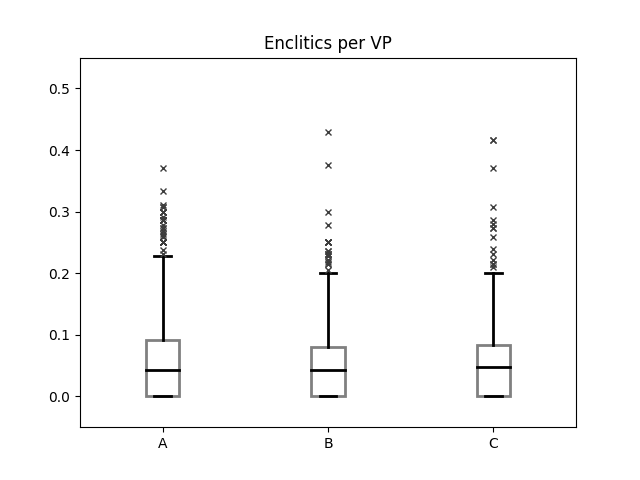
\includegraphics[width=0.9\linewidth]{images/enc.png}
\end{subfigure}%

\begin{subfigure}{1.0\textwidth}
  \centering
  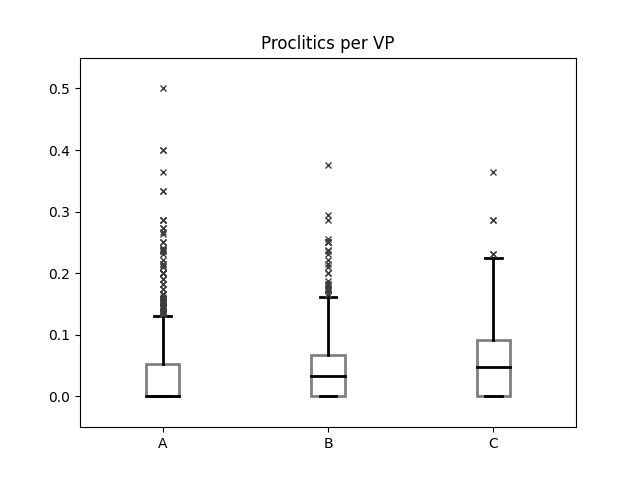
\includegraphics[width=0.9\textwidth]{images/proc.png}
\end{subfigure}
\caption{Use of clitic constructs in NLI-PT.}
\label{fig:clitics}
\end{figure}

It follows that the number of proclitics employed is better correlated with proficiency level than enclitic use, as indicated by CfsSubsetEval. This corroborates the claim that proclitics are acquired in a later stage of development \citep{flores2014, costa2015}.

Curiously, the elusive mesoclitic is absent from the feature list. Being restricted to the future and conditional tenses, there are fewer opportunities for its use. The arcane manner in which it must split a verbal stem from its inflection may also deter students, preferring instead the more familiar clitic varieties. Indeed, average use rates for mesoclitics are near-zero for all levels, with only a handful of outliers almost equally distributed across classes, negating any potential effect.

Moving on to verbal morphology, two inflectional paradigms of interest make an appearance in CfsSubsetEval: the subjunctive mood, a pattern difficult for many students learning Romance languages, and the extremely rare inflected infinitive, present in few other languages.

The inflected infinitive is an unusual form that allows for person and number agreement with an untensed verb. There is always a grammatically-licensed finite alternative, meaning their use is never mandatory \citep{iverson2008}. \Citet{rothman2010, rothman2013} have suggested that these patterns are acquired by late childhood, but may still cause problems even for adults who may accept certain pragmatic cues and draw inferences that alter the intended meaning of the utterance. Unfortunately, most research on this phenomenon have focused on monolingual native speakers in {\scshape l1} acquisition.

The usage distribution across proficiency levels in NLI-PT is seemingly random, with no general trend in increased usage for higher proficiency levels. It is possible that, since the first and third person singular forms are inflected with a null morpheme and are therefore homographs with each other as well as their uninflected form, this could be either unintended use by the student or even misidentified by the Stanza parser. These conjectures, however, still do not explain its predictive value according to CfsSubsetEval, other than the fact that it is not strongly correlated to other input variables.

Subjunctive, on the other hand, is much easier to interpret. Romance languages are well known for their extensive verbal morphology which can be overwhelming for students coming from an {\scshape l1} without such variation. Furthermore, this mood is employed in non-epistemic situations that would otherwise make use of the indicative. While commonly triggered by certain verbs such as \textit{querer} ``to want", it may be difficult to identify when required by less common or more opaque predicates \citep{flores2016, jesus2019}.

Beginner students are less likely to use the subjunctive, being introduced to it at an intermediate stage. This is clearly evident in the distribution in NLI-PI, illustrated in Figure~\ref{fig:subjunctive}. The vast majority of level A students do not use subjunctive at all, even though there are many outliers. However, the distribution between levels B and C are almost the same, though slightly less for the more advanced. This could be due to the fact that this mood is introduced and practiced more at the intermediate stage. The distribution indicates that it is a good proxy by which to discriminate between beginner texts and the higher levels.

\begin{figure}[H]
    \centering
    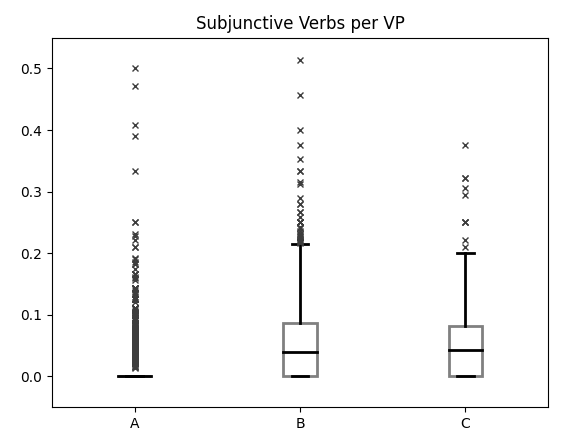
\includegraphics[width=0.8\textwidth]{images/svp.png}
    \caption{Use of subjunctive in NLI-PT.}
    \label{fig:subjunctive}
\end{figure}

The various clefting strategies available in Portuguese give rise to the potential for great syntactic variation. Of the five cleft constructions described in Section~\ref{section:pt}, only two were identified often enough in the corpus to make any impact: it-clefts and \textit{é que} clefts. \textit{WH}-clefts were not found at all, and the remaining pseudoclefts and inverted pseudoclefts were sparse. However, this may be the result of poor tagging and parsing of the learner texts using models trained on native text, and consequently the possibly unintuitive matching patterns described in Table~\ref{tab:tregex}, which were designed for the parsing model trained using simple left head-finding rules.

\Citet{lobo2015} found that both it-clefts and \textit{é que} clefts are acquired earlier than the remaining varieties and are generally widespread in child speech. In NLI-PT, standard clefts are used less frequently overall than \textit{é que} clefts, but the former is employed similarly across proficiency levels compared to the latter, which appears more often in higher proficiency levels. This also suggests that it is helpful in classifying higher levels compared to CEFR-A.

Interestingly, few features appear that target morphology, which would have been expected given the highly inflectional nature of Portuguese in addition to the results obtained by \cite{vajjala2014-estonian} for Estonian, which conclude that morphological features can be highly predictive. \Citet{delrio2019a}'s use of POS \textit{n}-grams with fine-grained morphological information seems to fill this gap, with \cite{vajjala2018-cefr} also observing promising results using word and POS \textit{n}-grams, though \cite{vajjala2014-estonian} reported low scores using POS \textit{n}-grams.

Encoding native language as a categorical feature has also been postulated to be a useful feature in proficiency classification \citep{vajjala2017-features}, but no information gain was observed in this study with the exception of Russian being the only one to appear as a viable {\scshape l1} feature. This is an interesting development, since certain vocabulary and syntactic choices may be characteristic of a particular {\scshape l1} and may have potential transfer effects. For example, Spanish speakers may be expected to produce a higher rate of grammatical sentences even at lower levels given the close proximity between the two languages. This substantiates \cite{crossley2011}, having shown homogeneity between learners of varying {\scshape l1}s.

\subsection{Comparisons}

\Citet{delrio2019a} in her first experiments with Portuguese proficiency classification found complexity measures, which she refers to as ``descriptive" features, among the weakest predictors, with the best scores being achieved using bag-of-words and POS \textit{n}-grams. However, the set of approximately 39 complexity features she used is much smaller than the amount employed in this study.

Later, \cite{delrio2019b} obtained generally poor results in her experiments training systems on Spanish for cross-lingual classification, though there are a few interesting takeaways. While bag-of-words, POS, and dependency linguistic features outperform complexity features, their interclass results are quite inconsistent with lows ranging from 0.19 F-1 macro for classifying CEFR-B with dependency n-grams, to 0.68 F-1 macro in CEFR-A using POS n-grams. CEFR-C was not able to be classified with these features at all, scoring 0.0 F1-macro across the board. Complexity features, however, are more stable: general measures scored a high of 0.60 F1-macro for A, with other subsets scoring between 0.40 and 0.48. Among levels B and C, F1 scores are almost the same for all subsets: 0.48-0.49 for B and 0.25-0.30 for C. This suggests that, while the small set of complexity features on their own may not have been the best, they are still insightful as predictive variables.

Combining these complexity measures with POS \textit{n}-grams resulted in further accuracy gains for classes A and B, though F1 scores for level C surprisingly plummeted back to 0.0. Given that the best results she observed for Spanish monolingual classification, however, were achieved through a combination of POS \textit{n}-grams and a larger amount of complexity features, it follows that using these in tandem for monolingual Portuguese classification could lead to improved scores.

\subsection{Detractors}
\label{section:detractors}

Recall that linguistic complexity and accuracy are separate entities in the CAF triad for measuring second language acquisition \citep{housen2009}. While complexity focuses on elaborateness and variation in learner expression, it is not concerned with errors made by students. However, the veracity of these feature calculations is susceptible to grammar and mechanical errors. Incorrect orthography or word choice obfuscates the student's intent, leading to incorrect tagging and parses and a contaminated analysis.

For example, one CEFR-A student achieved an impressive 50\% subjunctive verb usage per verb phrase, clearly visible in Figure~\ref{fig:subjunctive}. The subjunctive mood is often acquired later and it is therefore unlikely that a student would be capable of producing this construct so early, much less as often as was indicated. Upon closer inspection, it appears that this student—whose native language is Spanish—erroneously used the subjunctive present forms \textit{tome} and \textit{volte} instead of the indicative past \textit{tomei} and \textit{voltei}, which is clearly negative transfer from Spanish simple past, e.g. \textit{tomé}.

In the previous example, the verbal inflection was correctly identified, tagged, and parsed even though it was used incorrectly. Other situations result in a bad parse that propagates throughout the pipeline, culminating with an incorrect parse tree and, accordingly, inaccurate feature calculations. Sentence (\ref{sconj}) illustrates one such instance. The verb \textit{tendem} takes the optional prepositions \textit{a} or \textit{para} depending on context. This student has introduced an inappropriate preposition \textit{de} that is labeled by a confused tagger as a subordinate conjunction in what is really a simple sentence with no subordination.

\begin{exe}
\ex[*] {\label{sconj}
Os actores tendem de ser mais dramáticos também \\
The actors tend to to be more dramatic too}
\end{exe}

While Stanza otherwise provides a fairly competent parse of input text and relatively high accuracy is generally achieved for tokenization, tagging, lemmatization, and dependency parsing, there are still some shortcomings due to its data-driven approach and comparably smaller training set. For example, it seems that mesoclitics are not well-represented in the UD training corpus, because they are often poorly tokenized. This can be minor, as is the case with \textit{telefonar-lhes-ia} ``I would call them", which is split into \textit{telefonará} + \textit{lhes}, changing the tense from conditional to future. In other situations, it can result in very obscure results, such as merging an object pronoun with the inflected verb, introducing a new pronoun that was not present in the original mesoclitic, or even creating a brand new word not licensed by the language. This was resolved by creating hard-coded rules, searching for up to two object pronouns between hyphens and an inflectional suffix from one of the two appropriate tenses.

Another example would be the adverbial modifier ``how" and the first person singular conjugation of ``to eat", which are homonymous: \textit{como}. Only the former is represented in the UD training set which naturally leads to a questionable tag in a situation where the verb is clearly required. The parse tree for a sentence affected by this is depicted in Figure~\ref{fig:tree}.

\begin{figure}%[H]
\centering
    \tikzset{frontier/.style={distance from root=90pt}}
    \resizebox{\columnwidth}{!}{%
    \Tree[. \node{{\scshape s}}; 
        [. \node{{\scshape adv}}; 
        [. \node{\textit{Normalmente}}; ] ] 
        [. \node{{\scshape s}}; 
        [. \node{{\scshape np}}; 
        [. \node{{\scshape pron}}; 
        [. \node{\textit{eu}}; ] ] ]
        [. \node{{\scshape *s{\ \ }}}; 
        [. \node{{\scshape *pp{\ \ }}}; 
        [. \node{{\scshape *adp{\ \ }}}; 
        [. \node{\textit{como}}; ] ]
        [. \node{{\scshape np}}; 
        [. \node{{\scshape noun}};
        [. \node{\textit{torrada}}; ] ] ] ] 
        [. \node{{\scshape *s{\ \ }}}; 
        [. \node{{\scshape cconj}}; 
        [. \node {\textit{e}}; ] ]
        [. \node{{\scshape s}}; 
        [. \node{{\scshape vp}}; 
        [. \node{{\scshape verb}}; 
        [. \node{\textit{bebo}}; ] ] 
        [. \node{{\scshape np}};
        [. \node{$\overline{\mbox{{\scshape n}}}$};
        [. \node{{\scshape noun}}; 
        [. \node{\textit{café}}; ] ]
        [. \node{{\scshape pp}}; 
        [. \node{{\scshape adp}}; 
        [. \node{\textit{com}}; ] ] 
        [. \node{{\scshape np}}; 
        [. \node{{\scshape noun}};
        [. \node{\textit{leite}}; ] ] ] ] ] ] ] ] ] ] ] ]
        }
    \caption{Constituency tree for ``Normally I eat toast and drink coffee with milk". The verb \textit{como} ``eat" is mistaken for its prepositional homonym, projecting to a prepositional phrase instead of a verbal phrase. The error percolates to the sentence conjunct, which should be a complementizer phrase.}
    % Original text: \texttt{eng\_A\_031CVITF\_2\_cop.txt}.
    \label{fig:tree}
\end{figure}

Incorporating learner errors could provide a further dimension in which to better predict proficiency level. \Citet{vajjala2017-features, weiss2019-german} both found that errors in conjunction with complexity features were useful in their proficiency classification experiments. Further, \citet{delrio2019a} hypothesized that bag-of-words performed strongest for Portuguese proficiency classification because it can help identify orthographic mistakes. POS \textit{n}-grams, which were the next best feature in isolation, are also able to capture, for example, agreement errors in gendered nouns and adjectives. Both of these performed better in her experiments over the linguistic complexity features, so combining their effects with the augmented complexity feature set introduced in this work could be beneficial, as would incorporating other error patterns such as the incorrect expansion of mandatory contractions (see Section~\ref{section:pt}) and allomorphic variation of clitics.

Task variation may also negatively impact the classifier due to varied learner language across different prompts. As mentioned in Section~\ref{section:data}, texts are not labeled according to their associated topic and resolving topics from the texts themselves is non-trivial. Since linguistic complexity analyses are sensitive to the topic around which each text is based, as varied writing prompts can elicit different language patterns \citep{ventura2015, yang2015}, this has the potential to adversely influence the analysis because similar tasks cannot be grouped together during evaluation.

\subsection{Proficiency Levels}

Most other CEFR proficiency evaluations have determined that levels A and C classes are easier to classify, while this analysis observes C as being the hardest with A and B achieving similarly good results. NLI-PT has a large class imbalance, containing a similar number of entries for classes A and B, but roughly one third the amount of each for level C. \Citet{delrio2019a} accounts for this by performing trials on both the full dataset as well as a balanced subset, equally representing all classes. While predictions for C improve dramatically compared to other levels with the balanced set, it remains the class most often misclassified.

For a three-way classification problem with a random baseline of 33\%, complexity measures performed somewhat decently with consistent scores in the high 60\% accuracy range, rivaling the existing work performed by \cite{delrio2019a}. However, since proficiency level is measured on a spectrum, it follows that there is much overlap between adjacent levels, to say nothing of the variance caused by human error or bias when manually assigning levels. As such, it is of interest to visualize how closely these levels are at an empirical level.

Dimensionality reduction was conducted using principal component analysis with scikit-learn to inspect the trends between two automatically-extracted features that were deemed to be predictive of the target variable. Each feature group was performed separately, presented in Figure~\ref{fig:pca-sub}, in addition to the combined feature set, shown in Figure~\ref{fig:pca-all}. For surface, lexical, and morphosyntactic features, CEFR-A is the only group that appears to cluster somewhat distinctly. There is much overlap between CEFR-B and CEFR-C across all feature sets, explaining some of the difficulty in distinguishing them.

\begin{figure}[H]
\centering
\begin{subfigure}{0.5\textwidth}
  \centering
  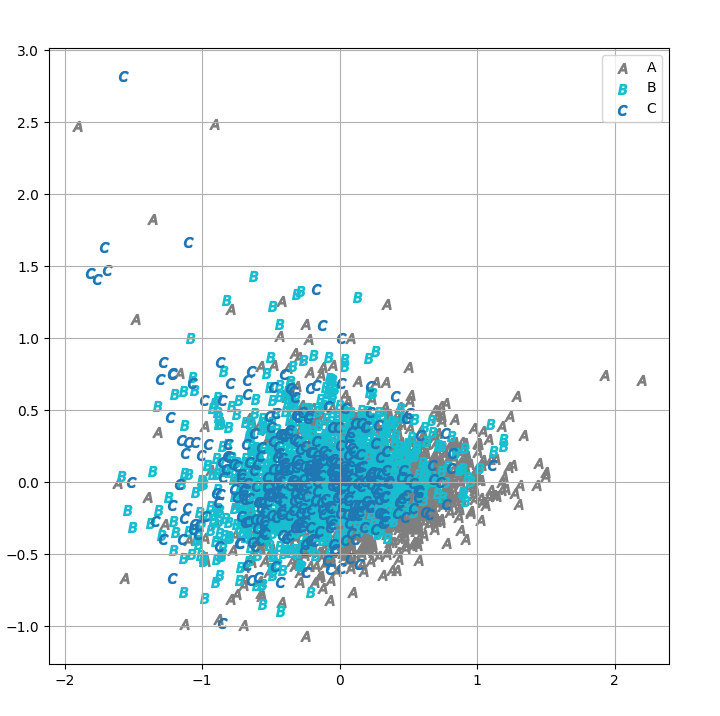
\includegraphics[width=1\linewidth]{pca-surface.png}
   \caption{Surface features.}
\end{subfigure}%
\begin{subfigure}{0.5\textwidth}
  \centering
  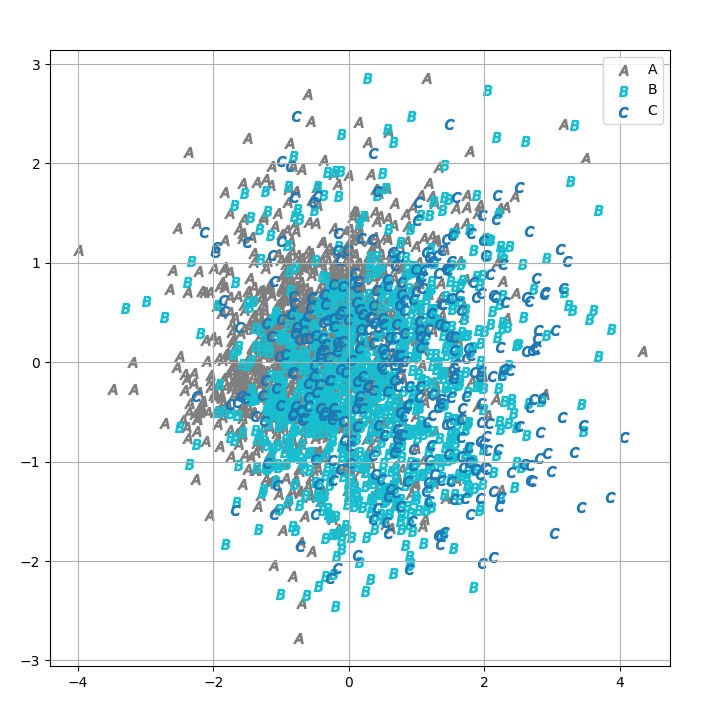
\includegraphics[width=1\linewidth]{pca-lexical.png}
  \caption{Lexical features.}
\end{subfigure}%

\begin{subfigure}{0.5\textwidth}
  \centering
  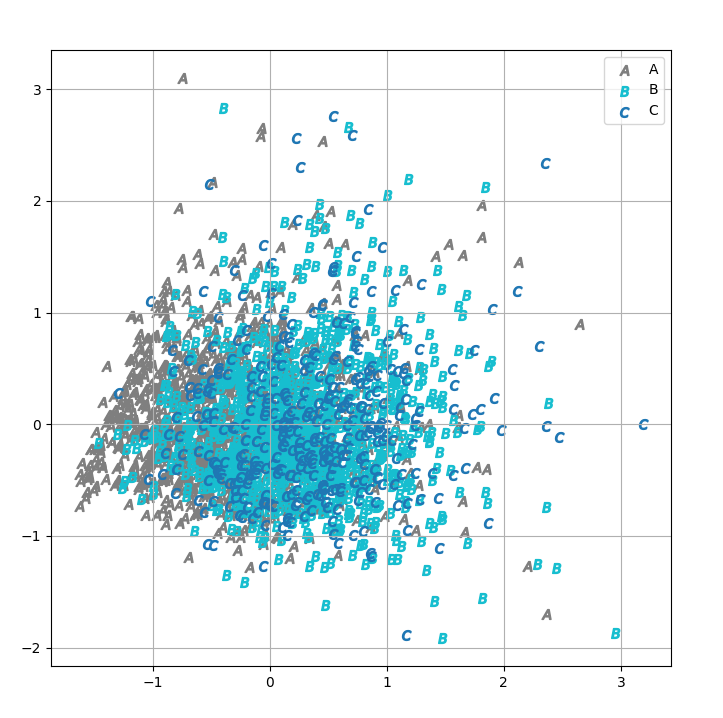
\includegraphics[width=1\linewidth]{pca-msy.png}
  \caption{Morphosyntactic features.}
\end{subfigure}%
\begin{subfigure}{0.5\textwidth}
  \centering
  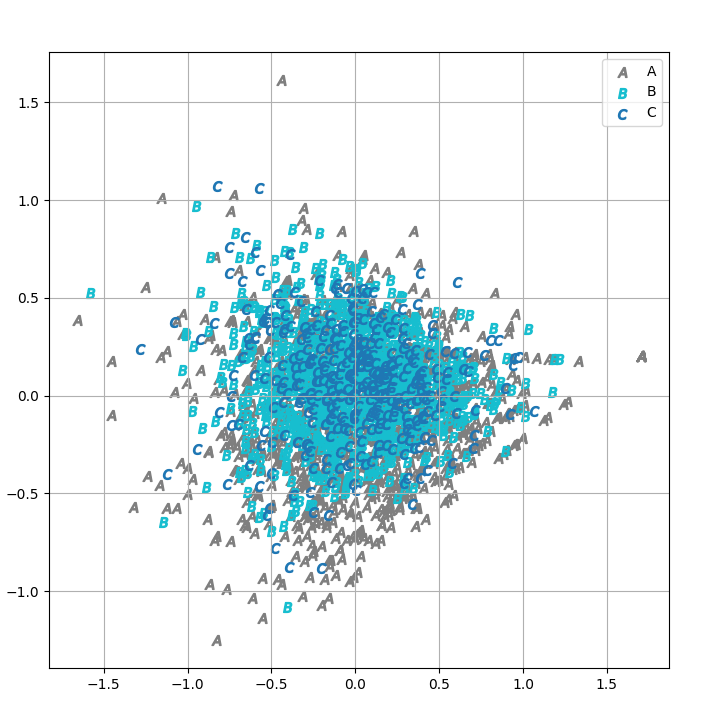
\includegraphics[width=1\textwidth]{pca-coh.png}
  \caption{Cohesion features.}
\end{subfigure}
\caption{Principal component analysis for different feature subsets.}
\label{fig:pca-sub}
\end{figure}


\begin{figure}[H]
    \centering
    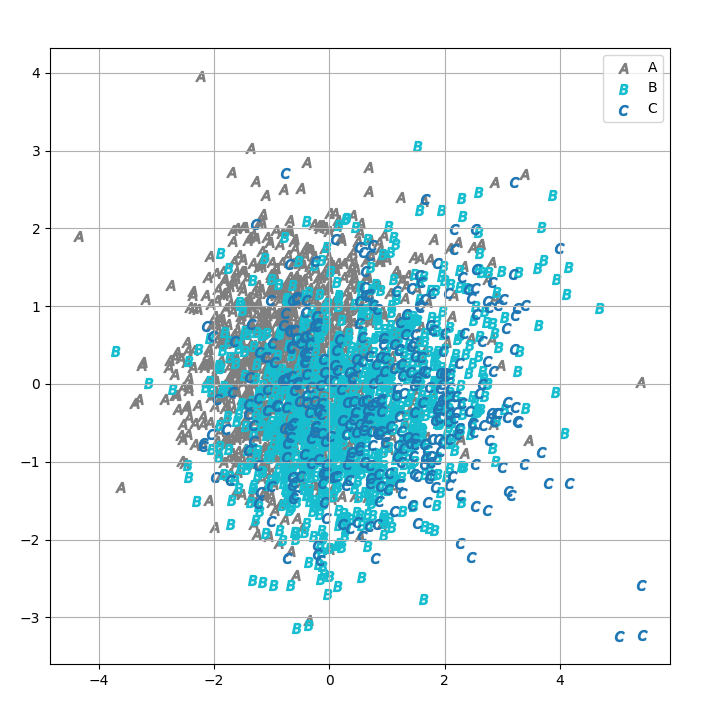
\includegraphics[width=1\linewidth]{images/pca-all.png}
    \caption{Principal component analysis for combined features.}
    \label{fig:pca-all}
\end{figure}
